\documentclass{article}
\usepackage[left=2cm,right=2cm,top=2cm,bottom=2cm]{geometry}
\usepackage[utf8]{inputenc}
\usepackage[german]{babel}
\usepackage{amsmath}
\usepackage{dsfont}
\usepackage[export]{adjustbox}
\usepackage{amsthm}
\usepackage{color}
\usepackage{amsfonts}
\usepackage{amssymb}
\usepackage{wasysym}
\usepackage{makeidx}
\usepackage{graphicx}
\usepackage[colorlinks=true,urlcolor=blue,linkcolor=blue]{hyperref}
\usepackage{ziffer}
\usepackage{minted}
\usepackage{xcolor}
\usepackage{framed}
\usepackage{mdframed}
\usepackage{subfiles}
\usemintedstyle{emacs}

\definecolor{purp}{HTML}{9A72AC}
\definecolor{re}{HTML}{FC6255}
\definecolor{gre}{HTML}{83C167}
\definecolor{blu}{HTML}{58C4DD}
\definecolor{shadecolor}{rgb}{0.85,0.85,0.85}
\definecolor{bg}{rgb}{0.95,0.95,0.95}
\setlength{\parindent}{0em} 

\BeforeBeginEnvironment{minted}{\begin{mdframed}[linewidth =2 ,backgroundcolor=bg , linecolor=black, linewidth=0.5]}
\AfterEndEnvironment{minted}{\end{mdframed}}

\newtheorem{defi}{Definition}
\BeforeBeginEnvironment{defi}{\begin{mdframed}[linewidth =2 ,backgroundcolor=bg , linecolor=black, linewidth=0.5]}
\AfterEndEnvironment{defi}{\end{mdframed}}

\newcommand{\bsp}{\textbf{Beispiel}:}
%\newcommand{\task}{\textbf{Aufgabe}:}

\newcommand{\bol}[1]{\textbf{#1}}
\newcommand{\q}[1]{\glqq #1\grqq}
\newcommand{\DODO}[1]{\textbf{\textcolor{red}{DODO:}} #1 \\ \begin{center}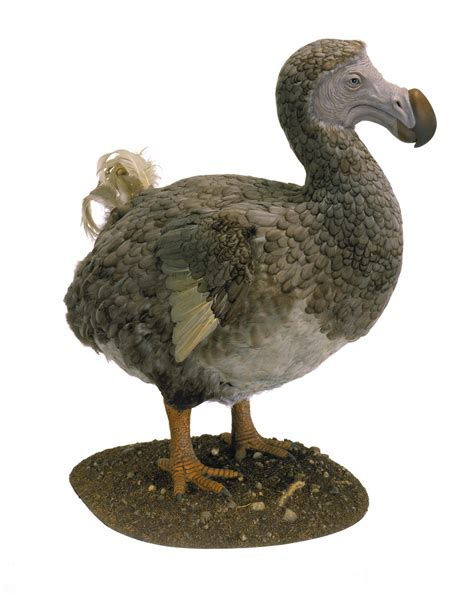
\includegraphics[scale=0.2]{../../media/dodo.jpg} \end{center}}

\newenvironment{task}[1]{
    \begin{shaded*}
    \textbf{Aufgabe #1}:
}{
    \end{shaded*}
}

\begin{document}
\begin{center}
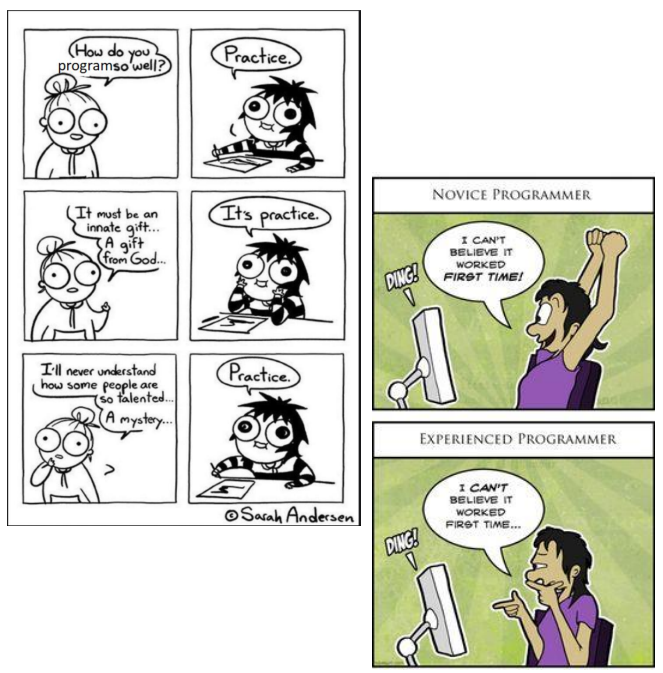
\includegraphics[scale = 0.8]{../../media/starting_cartoon.png}
\end{center}
\newpage
Gemeinhin ist eine Liste eine Aufzählung von Dingen, seien es Zahlen (Altersangaben einer Klasse), Worte 
(Einkaufszettel) oder eine Liste von Personen. 
\begin{itemize}
    \item Eier
    \item Mehl
    \item Salz
    \item Karrotten
\end{itemize}
\textbf{Listen} sind so alltäglich, dass wir überlicherweise gar nicht aktiv über sie nachdenken. \\
Unser erstes Ziel in diesem Schuljahr ist die Übertragung des Konzepts der Liste in die Informatik. 
Hier benötigen wir noch viel öfter \textbf{\q{Zusammenstellungen}} von Dingen.
Das Zusammenfassen von Objekten zu Listen ist sogar so zentral, dass es  Programmiersprachen gibt,
die auf die Liste als Basiselement zurückgreifen, z.B. Lisp. \\
Traditionell ist die Liste ein umso wichtigeres Element der Sprache, je funktionaler diese angelegt ist. In objektorientierten Sprachen sind Listen in ihrer Funktionalität zwar ebenfalls vorhanden, allerdings nicht immer ohne einen gewissen Aufwand zu verwenden. \\
In den folgenden Kapitel werden wir selbst Implementierungen für Listen in Java entwickeln. 
Wie oft in der Programmierung gibt es dabei \textbf{nicht} einen Königsweg, sondern
verschiedene Ansätze, die unterschiedliche Vor- und Nachteile bringen. \\
Als Prototyp einer Liste wird uns dabei eine \textbf{Warteschlange} dienen (ganz bildlich gedacht), z.B. die Schlange vor einer Kasse.
\begin{center}
    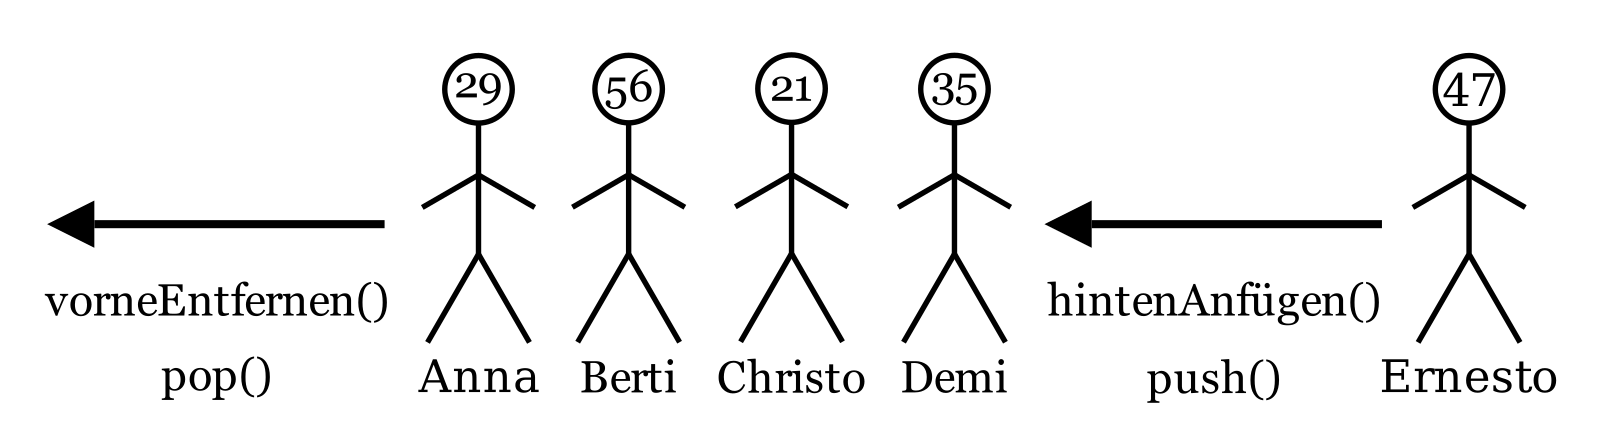
\includegraphics[scale=0.30]{../../media/queue.png}
\end{center}
\textbf{Hinweis:} Um sprachlich stringenter zu bleiben und Denglisch möglichst zu vermeiden, werden die Methoden im Fließtext häufig auf Deutsch stehen bzw. beschrieben werden, mit der üblichen englischen Übersetzung bei der ersten Verwendung in Klammern. Auch die Abbildungen werden, wenn nötig, beide Schreibweisen enthalten, der Quellcode aktuell nur englische Bezeichungen (Eine zweite Version des Skripts mit deutschem Quellcode ist geplant, wenn nötig). Für Prüfungen sind sowohl deutscher als auch englischer Quellcode in Ordnung.
Begründungen müssen aber in jedem Fall auf Deutsch geschrieben werden. Im Abitur ist auch der Quelltext i.d.R. auf Deutsch. \\
Zurück zum obigen Bild. Wir werden Anna, Berti, Christo, Demi und Ernesto noch öfter sehen, da sie unsere Liste füllen und auch wieder verlassen werden. 
Sie stehen in einer \textbf{Warteschlange (Queue)}. Auch eine Warteschlange ist nur eine Form von Liste, allerdings mit speziellen Eigenschaften.
Halten sich alle an die Regeln, so ist es nur möglich, dass sich jemand hinten anstellt oder vorne aus der Warteschlange entfernt wird, weil er dran ist und \q{abgearbeitet} wird. In unserer zukünftigen Modellierung entspricht dies den Methoden vorneEntfernen() (pop()) bzw. hintenAnfügen() (push()). \\
\textit{Hinweis:} Übergabeparameter werden im Text häufig weggelassen, natürlich müsste die zweite Methode etwa so aussehen: hintenAnfügen(Mensch mensch).
Die Warteschlange gehorcht dem sogenannten \textbf{FIFO-Prinzip} (First In, First Out). Neben diesem gibt es noch weitere Ansätze, siehe dazu auch Kapitel 6, das sich mit Typen von Listen beschäftigt. \\
Es bleibt abschließend die Frage, wie sich die Idee einer Warteschlange objektorientiert umsetzen lässt.
\newpage
\end{document}